%!TeX ts-program = xelatex
%!TeX encoding = utf-8 Unicode
\documentclass[ieeetran]{article}
\usepackage{amsmath, amssymb}
\usepackage{graphicx}
\usepackage{wrapfig}

\title{Investment and Financial Management \\Lecture Notes}
\author{Efe Kamasoglu}

\begin{document}

\maketitle

\pagebreak

\section{Introduction \& Financial Analysis} % (fold)
\label{sec:introduction_&_financial_analysis}

\textbf{Corporate Finance:}
Identifying profitable investment projects + Determining optimal financing + Liquidity planning
=> \underline{Maximizing firm / enterprise value}

\section{Financial Analysis} % (fold)
\label{sec:financial_analysis}



% section financial_analysis (end)

\subsection{Firms's disclosure of financial information} % (fold)
\label{sub:}



% subsection  (end)

\textbf{Purpose of financial statements:}
\begin{enumerate}
  \item Firm-issued accounting reports with past performance info
\item Reliable source of info for shareholders and stakeholders\footnote{A \textbf{shareholder} \underline{is someone who owns stock in your company}, while a \textbf{stakeholder} \textit{(example: supplier, government)} \underline{focuses on the company's overall performance}, how it treats customers, partners, and employees, and how it impacts the community, among other things.} of the firm
  \item Filed with relevant listing authority
  \item Preperation under certain rules and standards (GAAP, IFRS)
\end{enumerate}

\textbf{\\Main types of financial statements:}
\begin{enumerate}
  \item Balance sheet / statement of financial position
  \item Income Statement 
  \item Statement of cash flows
  \item Statement of changes in shareholders' equity
\end{enumerate}
 
\subsection{Balance sheet / statement of financial position} % (fold)
\label{sub:balance_sheet_statement_of_financial_position}

\textbf{Balance sheet / financial position:} snapshot of firm's financial position (assets, liabilities, shareholder's equity) at a given point in time

\textbf{\\Balance sheet equation:} Two sides must be equal: 
\underline{\textit{Assests = Liabilities + Shareholder's Equity}}

\begin{figure}[t]
  \centering
  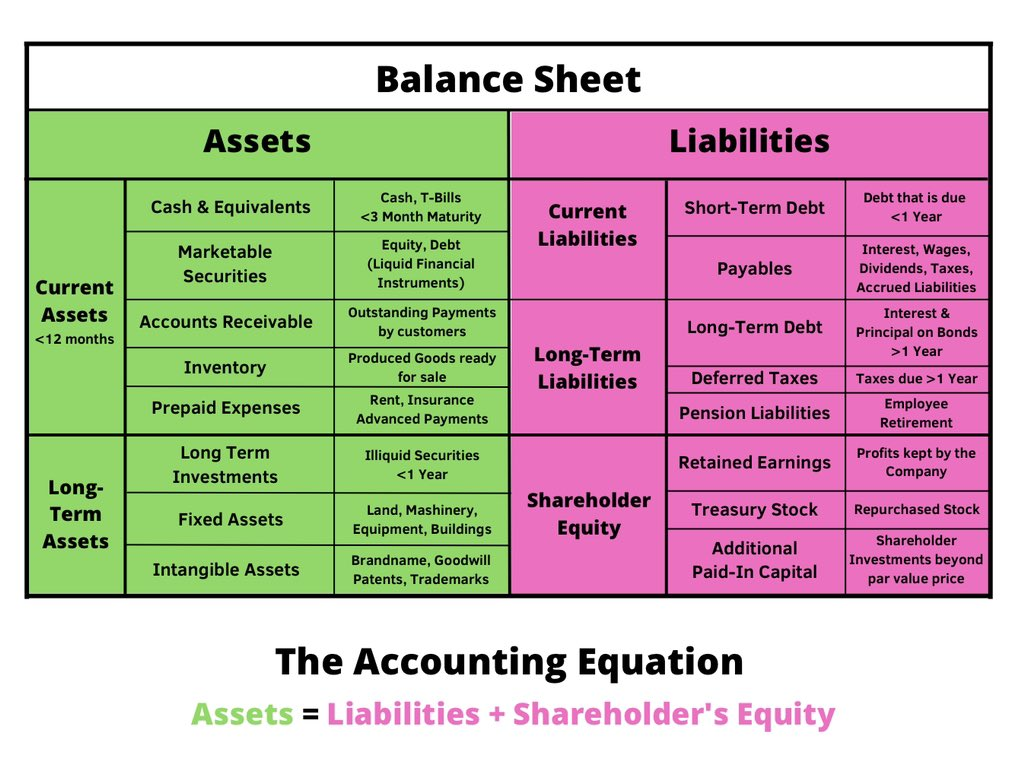
\includegraphics[width=0.58\linewidth]{balancesheet.jpg}
  \label{fig:balance_sheet_figure}
\end{figure}

\pagebreak

\begin{itemize}
  \item \textbf{Assets:} what the company owns
  \item \textbf{Liabilities:} what the company owes (debts, taxes etc.)
  \item \textbf{Shareholder's Equity:} difference between assets and liabilities
\end{itemize}

\begin{itemize}
  \item \textbf{Assets}
	\begin{itemize}
	  \item \textbf{Current Assests:} cash or expected to be turned into cash in the next year (not all operational!) \textit{(cash, marketable securities, accounts receivable, inventories)}
	  
	  \item \textbf{Non-current Assets (Fixed assets):} assets for long-term use (operational, more than one year) \textit{(net property, plant, equipment(PPE), goodwill and intangible assets)}
	\end{itemize}
   
\item \textbf{Liabilities}
	   \begin{itemize}
	     \item \textbf{Current Liabilities:} due to be paid within one year \textit{(accounts payable, short-term debt / notes payable, current maturities of non-current (long term) debt, taxes payable, wages payable)}
	     
	     \item \textbf{Net working capital (NWC):}
		     \large
		     \begin{equation*}
		     \boxed{NWC = Current \; Assets - Current \; Liabilities}
		     \end{equation*}
		     \normalsize
	     
	     \item \textbf{Non-current Liabilities:} to be paid beyond one year \textit{(long-term debt, capital leases, deferred taxes)}    
	   \end{itemize}

   \item \textbf{Shareholder's Equity: Book value vs. Market value}\footnote{\textbf{Book value} is the \underline{net value of a firm's assets} found on its balance sheet. \textbf{Market value} is the \underline{company's worth} based on the total value of its outstanding shares in the market, which is its market capitalization.}
	\begin{itemize}
	  \item \textbf{Book value of equity:}
		  \large
		  \begin{equation*}
		  \boxed{Book \; value \; of \; equity = 
		  Book \; value \; of \; assets - Book \; value \; of \; liabilities}
		  \end{equation*}
		  \normalsize
		  
		  \begin{itemize}
		    \item Could be negative
		    \item Many of the valuable assets may not be captured on the balance sheet	
		  \end{itemize}

	 \item \textbf{Market value of equity (= Market capitalization, market cap):}		 	 \large
		  \begin{equation*}
		  \boxed{Market \; value \; of \; equity = 
		  Market \; price \; per \; share * No. \; of \; shares \; outstanding}
		  \end{equation*}
		  \normalsize
		  \begin{itemize}
		    \item Cannot be negative
		    \item Often differs substantially from book value
		  \end{itemize}
	  
	  \item \textbf{Market-to-book (M/B) ratio (= Price-to-book (P/B) ratio):}
		 \large
		  \begin{equation*}
		  \boxed{M/B \; ratio = \frac{Market \; value \; of \; equity}{Book \; value \; of \; equity} 
		  }
		  \end{equation*}
		  \normalsize
		  \begin{itemize}
		    \item Successful firms have M/B ratio higher than 1
		    \item Value Stocks\footnote{A \textbf{value stock} is trading at levels that are \underline{perceived to be below its fundamentals}.}: Low M/B ratios
		    \item Growth stocks\footnote{A \textbf{growth stock} is any share in a company that is \underline{anticipated to grow} at a rate significantly above the average growth for the market \textit{(example: TSLA)}.}: High M/B ratios
		  \end{itemize}

  \end{itemize}
\item \textbf{Enterprise value (EV) (= Total enterprise value (TEV))}
	\begin{itemize}
	  \item Value of firm's underlying business operations / assets
	  \item Enterprise value $\neq$ Equity value 
		  \large
		  \begin{equation*}
		  \boxed{Enterprise \; value = 
		  Market \; value \; of \; equity + \underbrace{Debt - Cash}_\text{Net debt}}
		  \end{equation*}
		  \normalsize
	  \begin{itemize}
	  \item $Net \;  debt = Total \; debt - Cash \;  \& \; short\text{-}term \; investments$
	  \end{itemize}
subs
	\end{itemize}	
\end{itemize}


   

% subsubsection fdsfd (end)   
% subsubsection balance_sheet_statement_of_financial_position (end)
% subsubsection  (end)


% subsubsection firms_disclosure_of_financial_information (end)

% subsection  (end)


% section introduction_&_financial_analysis (end)

\subsection{Income statement} % (fold)
\label{sub:subsubName}
\textbf{Income statement:} record of a firm's revenue, expense, and profit over a given period of time

\pagebreak

\begin{figure}[t]
  \centering
  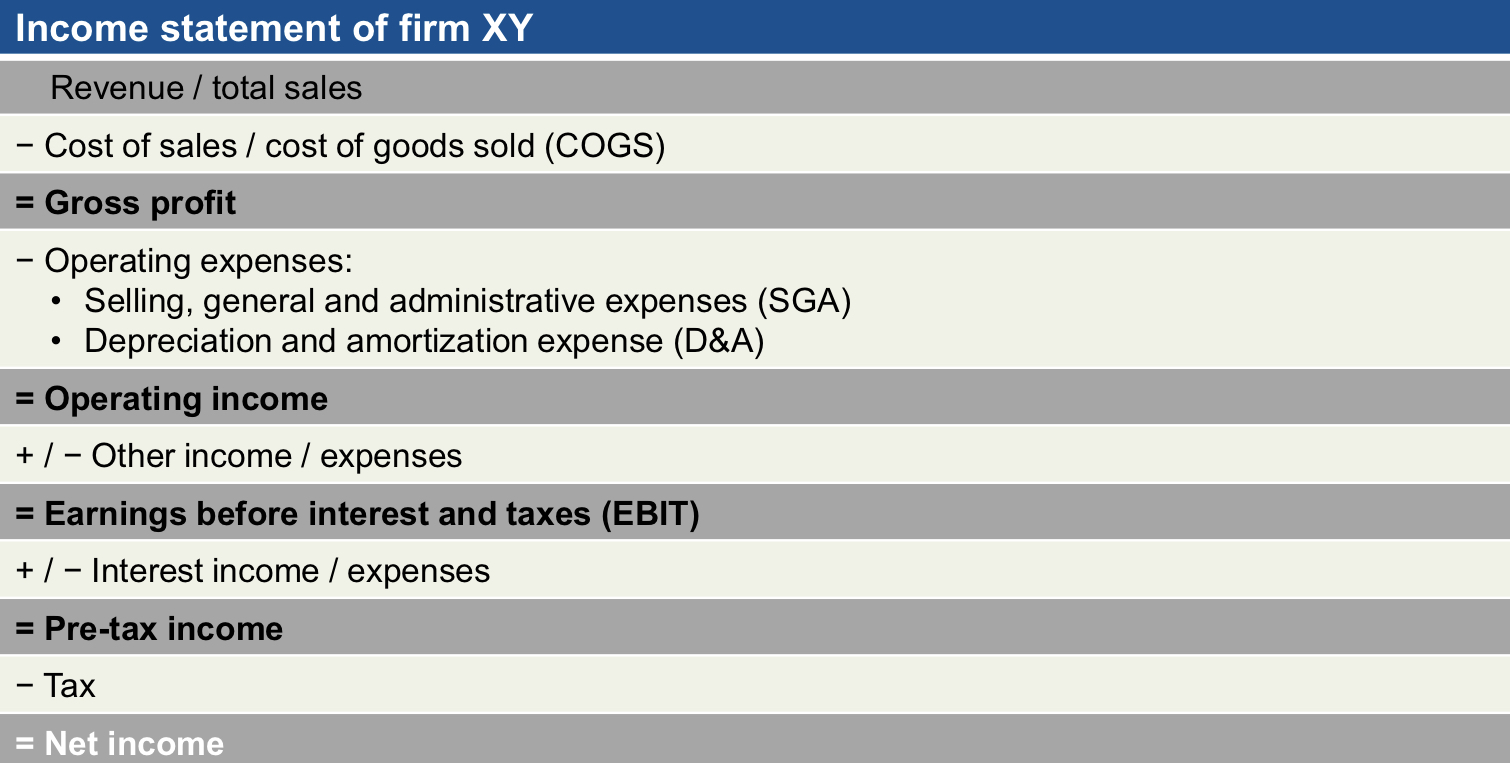
\includegraphics[width=1\linewidth]{incomestatement.jpg}
  \label{fig:income_statement_figure}
\end{figure}
\begin{itemize}
  \item \textbf{Net Income = Total earnings of the firm's equity holders}
	  \begin{itemize}
	    \item \textbf{Earnings per share (EPS):} how much money a company makes for each share of its stock
		   \large
		   \begin{equation*}
		   \boxed{EPS = \frac{Net \; income}{Shares \; outstanding}}
		   \end{equation*}
		   \normalsize

	   \item \textbf{Diluted earnings per share (Diluted EPS):}\footnote{\textbf{Dilution} occurs when a company \underline{issues new shares} that result in \underline{a decrease in existing stockholders' ownership percentage} of that company.} Future EPS could be diluted by in-the-money share (stock) options, convertible bonds or warrants. The diluted EPS takes these potential effects intp account.		   	

	  \end{itemize}

\end{itemize}

\subsection{Statement of cash flows} % (fold)
\label{sub:statement_of_cash_flows}
\begin{itemize}
  \item Record of sources and uses of the firm's cash over a given period of time
	  \begin{itemize}
	    \item Sources of cash: activity that brings cash into firm \textit{(example: sales)}
	    \item Uses of cash: causes cash to leave firm \textit{(example: dividend payments\footnote{A \textbf{dividend} is the \underline{distribution of a company's earnings to its shareholders} and is determined by the company's board of directors.})}
	  \end{itemize}
	    \item Derived from firm's income statement and changes in balance sheet
	    \item Consists of:
		    \begin{itemize}
		      \item Cash flows from \textbf{operating}, \textbf{investing} and \textbf{financing} activities
		    \end{itemize}
\end{itemize}

\pagebreak
 
\subsection{Financial statement analysis} % (fold)
\label{ssub:}
\begin{itemize}
  \item \textbf{Financial ratios}
	  \begin{itemize}
	    \item Are used to:
		    \begin{itemize}
		      \item Compare firm with itself over time
		      \item Compare firm to other similar firms
		    \end{itemize}
	    \item Key financial ratios measure a firm's:
		    \begin{itemize}
		      \item Profitability
		      \item Liquidity
		      \item Working Capital
		      \item Interest Covarage
		      \item Leverage (Gearing)
		      \item Valuation
		      \item Operating Returns 
		    \end{itemize}
	  \end{itemize}

 \item \textbf{Profitability ratios}
	 \begin{itemize}
		 \item Measures of a firm's ability to generate profits as a percentage of the sales generated (margin ratios; margin = portion of sales that is a profit)
		\item Four levels of profitability ratios (resulting from income statement)
			\begin{enumerate}
			  \item 
			  \large
			  \begin{equation*}
			  \boxed{Gross \; margin = \frac{Gross \; profit}{Sales}}
			  \end{equation*}
			  \normalsize
			  
			  \item 
			  \large
			  \begin{equation*}
			  \boxed{Operating \; margin = \frac{Operating \; income}{Sales}}
			  \end{equation*}
			  \normalsize

			  \item 
			  \large
			  \begin{equation*}
			  \boxed{EBIT \; margin = \frac{EBIT}{Sales}}
			  \end{equation*}
			  \normalsize

			  \item 
			  \large
			  \begin{equation*}
			  \boxed{Net \; profit \; margin = \frac{Net \; income}{Sales}}
			  \end{equation*}
			  \normalsize
	  \end{enumerate}

	 \end{itemize}

\item \textbf{Liquidity ratios}
	\begin{itemize}
	  \item Measures of a firm's ability to meet short-term debt obligations
	  \item Help to assess firm's liquidity / financial solvency info of balance sheet / statement of financial position
	  \begin{enumerate}
	    	\item 
		\large
		\begin{equation*}
		\boxed{Current \; ratio = \frac{Current \; assets}{Current \; liabilities}}
		\end{equation*}
		\normalsize

	    	\item 
		\large
		\begin{equation*}
		\boxed{Quick \; ratio = \frac{Cash + Short\text{-}term \; investm. + Accounts \; receivables}{Current \; liabilities}}
		\end{equation*}
		\normalsize

	    	\item 
		\large
		\begin{equation*}
		\boxed{Cash \; ratio = \frac{Cash}{Current \; liabilities}}
		\end{equation*}
		\normalsize
	  \end{enumerate}
	\end{itemize}

\item \textbf{Interest coverage ratios}
	\begin{itemize}
	  \item Measures of a firm's ability to meet its interest payments by comparing its earnings with its interest expenses
	  \item Higher ratio = firm is earning much more than necessary to meet its obligations
	\end{itemize}
	  \begin{enumerate}
	    \item
	    \large
	    \begin{equation*}
	    \boxed{EBIT/Interest \; coverage = \frac{EBIT}{Interest \; expense}}
	    \end{equation*}
	    \normalsize

	    \item
	    \large
	    \begin{equation*}
		    \boxed{EBITDA/Interest \; coverage = \frac{\overbrace{EBITDA}^\text{EBIT + Depreciation/Amortization\footnotemark}}{Interest \; expense}}
	\end{equation*}
	  \normalsize

 
\end{enumerate}

\footnotetext{\textbf{Amortization} is the method that is used to \underline{decrease the cost of the asset over time}, while \textbf{depreciation} is the \underline{loss in value of the asset over time}. Both of them are methods of calculating the value for business assets over time.}

\item \textbf{Leverage / gearing ratios}
	\begin{itemize}
		\item Measures of a firm's reliance on debt as a source of financing
		\item Leverage ratios can be measured using book or market values!
          	\item Important and common ratios:
			\pagebreak
			\begin{enumerate}
	    			\item
	    			\large
	    			\begin{equation*}
					\boxed{Debt\text{-}equity \; ratio = \frac{Total \; debt}{Total \; equity}}
	   			\end{equation*}
	    			\normalsize 
				 
	    			\item
	    			\large
	    			\begin{equation*}
					\boxed{Debt\text{-}to\text{-}capital \; ratio = \frac{Total \; debt}{Total \; equity + Total \; debt}}
	   			\end{equation*}
	    			\normalsize

	    			\item
	    			\large
	    			\begin{equation*}
					\boxed{Debt\text{-}to\text{-}EV \; ratio = \frac{Net \; debt}{Market \; value + Net \; debt}}
	   			\end{equation*}
	    			\normalsize

	    			\item
	    			\large
	    			\begin{equation*}
					\boxed{Equity \; multiplier = \frac{Total \; assets}{Book \; value \; of \; equity}}
	   			\end{equation*}
	    			\normalsize
			\end{enumerate}
	\end{itemize}

\item \textbf{Valuation ratios}
	\begin{itemize}
	  \item Measures to help investors assess market value of a firm
	  \item These ratios are intended to make intra-industry comparisons of firm valuations.
	  \begin{enumerate}
	    \item
	    \large
	    \begin{equation*}
		    \boxed{
			\begin{aligned}
		    Price\text{-}to\text{-}earnings \; (P/E) \; ratio = \frac{Market \; capitalization}{Net \; income}\\
		    \\
		    = \frac{Share \; price}{Earnings \; per \; share}
			\end{aligned}
	    }
	    \end{equation*}
	    \normalsize

	    			\item
	    			\large
	    			\begin{equation*}
					\boxed{EV \; to \; EBIT = \frac{Market \; value \; of \; equity + Debt - Cash}{EBIT}}
	   			\end{equation*}
	    			\normalsize

	    			\item
	    			\large
	    			\begin{equation*}
					\boxed{EV \; to \; Sales = \frac{Market \; value \; of \; equity + Debt - Cash}{Sales}}
	   			\end{equation*}
	    			\normalsize				
	    
	  \end{enumerate}
	\end{itemize}

\item \textbf{Operating returns / investment returns}
	\begin{itemize}
	  \item Measures of a firm's returns on investment
       	  \item Compare its income to its investment using financial information from balance sheet / statement of financial position
		  \begin{enumerate}
		    \item 
		    \large
		    \begin{equation*}
		    \boxed{Return \; on \; equity \; (ROE)=\frac{Net \; income}{Book \; value \; of \; equity}}
		    \end{equation*}
		    \normalsize

		    \item 
		    \large
		    \begin{equation*}
		    \boxed{Return \; on \; assets \; (ROA)=\frac{Net \; income + Interest \; expense}{Total \; assets}}
		    \end{equation*}
		    \normalsize

		    \item 
		    \large
		    \begin{equation*}
		    \boxed{Return \; on \; invested \; capital \; (ROIC)=\frac{EBIT *  (1-Tax \; rate)}{Book \; value \; of \; equity + Net \; debt}}
		    \end{equation*}
		    \normalsize		    

		    \item 
		    \large
		    \begin{equation*}
		    \boxed{Asset \; turnover = \frac{Sales}{Total \; assets}}
		    \end{equation*}
		    \normalsize
		  \end{enumerate}
	\end{itemize}
\item \textbf{DuPont identity}
	\begin{itemize}
	  \item DuPont identity further decomposes return on equity (ROE) into theree components:
		  \begin{itemize}
		    \item Profitability (= Net profit margin)
	            \item Asset efficiency (= Asset turnover)
		    \item Leverage (= Equity multiplier)
			    \large
			    \begin{equation*}
				    \boxed{ROE = \underbrace{(\frac{Net \; income}{Sales})}_\text{Net profit margin} * \underbrace{(\frac{Sales}{Total \; assets})}_\text{Asset turnover} * \underbrace{(\frac{Total \; assets}{Book \; value \; of \; equity})}_\text{Equity multiplier}}
			    \end{equation*}
			    \normalsize
			    
		  \end{itemize}
	\end{itemize}
\end{itemize}
	
\section{Investment Analysis} % (fold)
\label{sec:investment_analysis}

\subsection{Net present value (NPV)} % (fold)
\label{ssub:net_present_value_nPV_}

\begin{itemize}
  \item \textbf{NPV (of a project or investment):} difference between present value of its benefits (cash inflow) and present value of its costs (cash outflow)

\large
\begin{equation*}
\boxed{
\begin{aligned}
NPV = PV(Benefits) - PV(Costs) =PV(All \; project \; cash \; flows)
\end{aligned}
}
\end{equation*}

\large
\begin{equation*}
\boxed{
\begin{aligned}
	NPV = \sum_{t=0}^{T} \frac{CF_t}{(1 + r)^t} 
\end{aligned}
}
\end{equation*}
\\
\normalsize
With:
\begin{itemize}
	\item NPV = Net present value, PV = Present Value, CF\textsubscript{t} = cash flow in period t, r = Appropriate discount rate
\end{itemize}

\item \textbf{NPV rule:}
	\begin{itemize}
	  \item \textbf{NPV decision rule:} When making an investment decision, take the alternative with the highest NPV.
     	  \item \textbf{Accepting or rejecting a project:}
		  \begin{itemize}
		    \item \underline{Accept, if positive NPV, expected profit} => equivalent to receiving its NPV cash today
		    \item \underline{Reject, if negative NPV, expected net loss} => would reduce the wealth of investors

		  \end{itemize}
	  \item \textbf{Alternative rules versus NPV rule:}
		  \begin{itemize}
		    \item Sometimes alternative investment rules give the same answer as the NPV rule, but at other times they disagree. \underline{If rules conflict, follow NPV decision rule.}
		    \item Equivalent rules: Economic value added (EVA), Annuity-rule
		  \end{itemize}
	\end{itemize}
\end{itemize}

\subsection{Internal rate of return (IRR)} % (fold)
\label{ssub:internal_rate_of_return_iRR_}
\begin{itemize}
  \item \textbf{IRR:} discount rate that makes NPV equal to zero (at which PV(Costs) = PV(Benefits))
	  \large
	  \begin{equation*}
	  \boxed{
	  \begin{aligned}
	  NPV = \sum_{t=0}^{N} \frac{CF_T}{(1+IRR)^t} = 0  
	  \end{aligned}
	  }
	  \end{equation*}
	  \\
	  \normalsize

	  With:
	  \begin{itemize}
	    \item NPV = Net present value, CF\textsubscript{t} = cash flow in period t,
		    IRR = Internal rate of return
	  \end{itemize}

\item \textbf{IRR rule:}
	\begin{itemize}
	  \item \textbf{IRR investment rule:}
		  \begin{itemize}
			  \item \underline{Take any investment, if its IRR exceeds cost of capital}\footnote{\textbf{Cost of capital} is the minimum rate of return or \underline{profit a company must earn before generating value} (e.g.\ undertaking a project, such as building new factory).}
			\item \underline{Turn any down investment, if its IRR is less than cost of capital}
		  \end{itemize}
	  \item \textbf{Application of IRR rule: IRR vs. NPV}
		  \begin{itemize}
			  \item IRR rule works for a stand-alone project if all of the project's \textbf{negative cash flows}\footnote{outgoing > incoming} precede \textbf{positive cash flows}\footnote{outgoing < incoming}. In other cases, \underline{IRR rule may disagree with NPV rule} thus be \underline{incorrect}!\\ 

			 \underline{\textit{Example:}}  \textit{If market conditions change over the years, project A can have multiple IRRs. Thus, IRR cannot be used. Instead, use NPV for comparison of projects.}
	
		  \end{itemize}
	  \item \textbf{Pitfalls of IRR rule:} Situations where IRR and NPV rules may conflict:
		\begin{enumerate}
		  \item Delayed investments
			  \item Multiple IRRs
				  \item Nonexistent IRR
		\end{enumerate}
		  \end{itemize}

\item \textbf{IRR vs. IRR rule:}
	\begin{itemize}
	  \item While IRR rule has shortcomings for making investment decisions, IRR itself remains useful.
	\item \textbf{But:}
		\begin{itemize}
		  \item IRR measures average return of investment => exact measure for average ROIC  of a project over its lifetime.
		  \item IRR can be used to check the sensitivity of NPV to any estimation error in the cost capital.
		\end{itemize}
	\end{itemize}
\item \textbf{Mutually exclusive projects:}
	\begin{itemize}
		\item When you must choose only one project among several possible projects, the choice is mutually exclusive\footnote{If two or more events are \textbf{mutually exclusive}, they \underline{cannot happen simultaneously}.}.
			\begin{itemize}
			  \item \underline{\textbf{NPV rule:}} Select the project with highest NPV.

			  \item \underline{\textbf{IRR rule:}} Selecting the project with the highest IRR may lead to mistakes.
			\end{itemize}
	\end{itemize}

\item \textbf{IRR rule and mutually exclusive investment with project ranking with different scales:}
	\begin{itemize}
	  \item If a project's size is doubled, its NPV will double. This is not the case with IRR. Thus, IRR rule cannot be used to compare projects of different scales.
	\end{itemize}

\item \textbf{Project ranking with timing of cash flows:}
	\begin{itemize}
	\item Problem with IRR: it can be affected by changing the timing of cash flows, even when the scale is the same.
	\item IRR is a return, but the dollar value of earning a given return depends on how long the return is earned.
	\item \underline{\textit{Example:}} \textit{A project with lower IRR can have a much higher NPV due to its higher growth rate.}
	\end{itemize}

\item \textbf{Project ranking with differences in risk:}
	\begin{itemize}
	  \item An IRR, that is attractive for a safe project, need not to be attractive for a riskier project.
	\item \underline{\textit{Example:}} \textit{IRR of a project is higher than those of the other investment opportunities, yet has the lowest NPV.}
	\item Higher cost of capital (e.g. due to size of the project) = Higher IRR
	\end{itemize}

\end{itemize}

\subsection{Other methods} % (fold)
\label{ssub:other_methods}

\begin{itemize}
\item \textbf{Payback method:}
	\begin{itemize}
	 \item \textbf{Payback period:} amount of time it takes to recover or pay back the initial investment (initial cash outflow).
\item \textbf{Payback rule:} \underline{Accept project}, if payback period is less than a pre-specified length of time. \underline{Otherwise reject}.

\item \textbf{Applicability of payback rule:} Payback rule is used by many companies due to its simplicity. Maybe, firms often care more about the liquidity drain of a project rather than its profitibility.

\item \textbf{Shortcomings of the payback rule:}
	\begin{itemize}
		\item Ignores the project's cost of capital and time value of money
			\footnote{\textbf{Time value of money} means that a sum of money is worth more now than the same sum of money in the future.\
			It can grow only \underline{through} \underline{investing so a delayed investment is a lost opportunity}.}
	\item Ignores cash flows after the payback period
	\item Relies on an ad hoc decision criterion
	\end{itemize} 
	\end{itemize}
 
\item \textbf{Probability index (PI):} PI can be used to identify the optimal combination of projects to undertake. Companies use it for evaluation of projects with different resource constraints.
	\large
	\begin{equation*}
	\boxed{
	\begin{aligned}
	Profitability \; index = \frac{Value \; created}{Resource \; consumed} = \frac{NPV}{Resource \; consumed}
	\end{aligned}
	}
	\end{equation*}
	\normalsize
\begin{itemize}
	\item \textbf{PI rule:} When choosing among projects competing for the same resource, pick the set of projects with the highest PIs that can still be undertaken given the limited resource.

\end{itemize}
\item \textbf{Shortcomings of PI:}
	\begin{itemize}
	  \item It does not take into account the size of the project, so it is not accurate in some cases.
	\item \underline{\textit{Example:}} \textit{A large project with lower profit margins may have a lower profitability index than a smaller project with higher profit margins.}
	\item Different combinations must be enumerated in order to find out NPV maximizing combination.
	\item With multiple resource constraints, PI can break down completely.
	\end{itemize}

\end{itemize}

\section{Capital Budgeting} % (fold)
\label{sub:capital_budgeting}
\textbf{Capital Budgeting:} A planning process used by a firm to determine if major projects or investments are worth the funding of cash capitalization structures (debt, equity or retained earnings)

\subsection{Determining free cash flow (FCF) and NPV} % (fold)
\label{ssub:determining_free_cash_flow_fCF_and_nPV}

\begin{itemize}
  \item \textbf{FCF:} It is the cash a company generates after taking into consideration cash outflows that support its operations and maintain its capital assets. Thus, it is firm's extra cash after its operating expenses and other areas.

  \item \textbf{Methods of calculation of free cash flow:}
	  \begin{itemize}
	    \item Direct calculation
	\item Calculation from earnings
	  \end{itemize}

\item \textbf{Two forms of free cash flow:}
	\begin{itemize}
	  \item \textbf{Free cash flow to the firm (FCFF):} FCF available to all providers of a firm's capital, including bondholders, shareholders and common stockholders.
	  \item \textbf{Free cash flow to the equity (FCFE):} FCF available to a firm's common (equity) stockholders
	\end{itemize}

\item \textbf{Direct calculation of FCF:}
	\large
	\begin{equation*}
	\boxed{
	\begin{aligned}
	FCF = \overbrace{(Revenue - Cost - Depreciation) * (1 - t_C)}^\text{Unlevered net income} + Depreciation - CapEx \\
	- \Delta NWC
	\end{aligned}
	}
	\end{equation*}
	\normalsize

	\large
	\begin{equation*}
	\boxed{
	\begin{aligned}
	FCF = (Revenue - Cost) * (1 - t_C) -CapEx - \Delta NWC + t_C * Depreciation
	\end{aligned}
	}
	\end{equation*}
	\\
	\normalsize
	With:
	\begin{itemize}
		\item FCF = Free cash flow, t\textsubscript{C} = Corporate tax rate, t\textsubscript{C} * Depreciation tax shield, CapEx = Capital expenditures, NWC = Net working capital
	\end{itemize}

\item \textbf{Calculation of FCF from earnings:}
	\begin{figure}[h!]
	  \centering
	  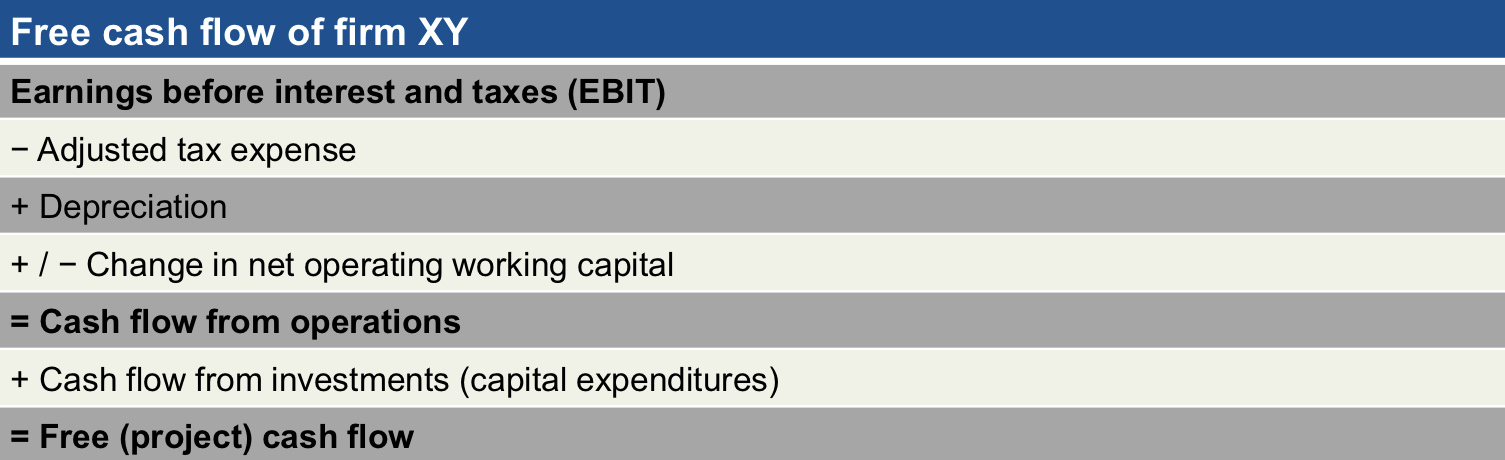
\includegraphics[width=1.0\linewidth]{FCFearnings.jpg}
	  \label{fig:fCFearnings_jpg}
	\end{figure}

\item \textbf{Forecasting earnings:}
	\begin{itemize}
	  \item \textbf{Capital budget:} Lists the investments that a company plans to undertake
	  \item \textbf{Capital budgeting:} Process used to analyze alternate investments and decide which ones to accept => \underline{using NPV to evaluate capital budgeting decisions}
	  \item \textbf{Incremental earnings:}  Amount by which the firm's earnings are expected to change as a result of the investment decision
 
	\end{itemize}
\item \textbf{Interest expense:}
	\begin{itemize}
		\item In capital budgeting decisions, \textbf{interest expense}\footnote{An \textbf{interest expense} is the cost incurred by an entity for borrowed funds.} is typically not included. Project should be judged on its own, not on how it will be financed.
			\item \textbf{Note:}
				\begin{itemize}
				  \item Interest expense is taken into account in cost of capital, i.e.\ discount rate used for calculating NPV.
				\item Hence, if we considered interest payments as an expense, there would be a \textbf{double counting}.
				\end{itemize}
	\end{itemize}
	\item \textbf{Tax considerations:}
		\begin{itemize}
			\item \textbf{Marginal corporate tax rate:} The tax rate on the marginal or incremental dollar of pre-tax income. \textbf{Note:} A negative tax is equal to a tax credit\footnote{\textbf{Tax credit} refers to an amount of money that taxpayers can subtract directly from the taxes they owe.}.
				\large
				\begin{equation*}
				\begin{aligned}
				\boxed{
				Income \; tax = EBIT * t_C
				}
			\end{aligned}
				\end{equation*}
				\normalsize
			
			\item \textbf{Note:}
				\begin{itemize}
				  \item Taxes paid by the company are lower as interest payment can be deducted from the tax base.
				  \item However, this \textbf{tax shield effect}\footnote{\textbf{Interest Tax Shield} refers to the tax savings \underline{resulting from the tax-deductibility of the} \underline{interest expense} on debt borrowings.} is taken into account in adjusting the cost of capital.
				\item Tax shield effect while calculating project's cash flows => there would be double counting 
				\end{itemize}
		\end{itemize}
\item \textbf{Tax credit:}
	\begin{itemize}
	  \item \textbf{Rationale:} Typically, in a new project, EBIT may be negative over the first years.
	  \item \textbf{Profitable company:}
		  \begin{itemize}
		    \item If the project takes place within an overall profitable company, we can calculate with negative tax payments, i.e.\ \underline{company is} \underline{granted a tax credit}.
		\item \underline{Reason:} The loss in project can be balanced against profits made in other business segments.
		  \end{itemize}
	\item \textbf{Non-profitable company:}
		\begin{itemize}
			\item If the overall company is not profitable, we have to set-up a tax carryforward\footnote{A \textbf{tax loss carryforward} allows taxpayers to use a taxable loss in the current period and apply it to a \underline{future tax period}.\ \textit{Result in the future}: decrease in taxable income (taxable income - carried taxable loss) => lower amount of tax} or (if allowed) a carrybackward.
		\end{itemize}
	\end{itemize}
\item \textbf{Opportunity cost:} It is the forgone benefit that would have been derived from an option not chosen.

\item \textbf{Project externalities:} Indirect effects of the project that may affect the profits of other business activities of the firm. \textbf{Cannibalization} is when sales of a new product displaces sales of an existing product.

\item \textbf{Sunk costs:} costs that have been or will be paid regardless of the decision whether or not the investment is undertaken -> not to be included in incremental earnings analysis!
	\begin{itemize}
	  \item \textbf{Overhead costs:} fixed and not incremental to the project
	  \item \textbf{Past research and development expenditures:} Money that has already been spent on R\&D is a sunk cost.
  \item \textit{They are both irrelevant for incremental (earning) analysis!} 
	  \item \underline{\textit{Reason:}} \textit{The decision to continue or abandon a project should be based only on the incremental costs and benefits of the product going forward.}
	\end{itemize}

\item \textbf{Unavoidable competitive effects:}
	\begin{itemize}
	  \item When developing a product, firms may be concerned about the cannibalization of existing products.
	\item If sales are likely to decline in any case as a result of new products introduced by competitors => these lost sales are a \textbf{sunk cost}
	\end{itemize}

\item \textbf{Real-world complexities:}\\
	\\Typically,
	\begin{itemize}
	  \item sales will change from year to year
	\item average selling price will vary over time
        \item average cost per unit will change over time
	\end{itemize}

\item \textbf{Capital expenditures and depreciation:}
	\begin{itemize}
	  \item \textbf{Capital expenditures:} Actual cash outflows when an asset is purchased -> included in calculating free cash flow
	  \item \textbf{Depreciation:} Non-cash expense\footnote{\textbf{Non-cash expenses} are business expenses that do not require the expenditure of cash. They do not have an effect on cash flow!} -> free cash flow estimate is adjusted for this non-cash expense
	\end{itemize}

\item \textbf{Net (operating working capital (NWC):)}
	\begin{itemize}
	  \item Most projects will require an investment in NWC.
		  \large
		  \begin{equation*}
		  \boxed{
		  \begin{aligned}
		  NWC = Current \; assets - Current \; liabilities
		  \end{aligned}
		  }
		  \end{equation*}
		  \normalsize
		  \large
		  \begin{equation*}
		  \boxed{
		  \begin{aligned}
		  NWC = Cash + Inventory + \underbrace{Receivables - Payables}_\text{Trade credit}
		  \end{aligned}
		  }
		  \end{equation*}
		  \normalsize
\item Increase in NWC:
	\large
	\begin{equation*}
	\boxed{
	\begin{aligned}
	\Delta NWC_t = NWC_t - NWC_{t-1}
	\end{aligned}
	}
	\end{equation*}
	\normalsize		  
	\end{itemize}

\item \textbf{Calculation of NPV:}
	\large
	\begin{equation*}
	\boxed{
	\begin{aligned}
		PV(FCF_t) = \frac{FCF_t}{(1+r)^t} = FCF_t * \frac{1}{(1+r)^t}
	\end{aligned}
	}
	\end{equation*}
	\normalsize
	
\end{itemize}

\subsection{Choosing among alternatives} % (fold)
\label{sub:choosing_among_alternatives}
\begin{itemize}
  \item \textbf{Rules for choosing among alternative projects:}
	  \begin{itemize}
	    \item \textbf{Choosing between mutually exclusive investment opportunities:} Pick the opportunity with highest NPV
    \item \textbf{Choosing between alternatives:} Only include those components of free cash flow that differ among the alternatives.
	  \end{itemize}
\end{itemize}

\subsection{Further adjustments to FCF} % (fold)
\label{sub:further_adjustments_to_fCF}
\begin{itemize}
  \item \textbf{Adjustments to FCF:}
	  \begin{itemize}
	    \item \textbf{Other non-cash items:} Amortization
	\item \textbf{Timing of cash flows:} Cash flows are often spread throughout the year
		\item \textbf{Accelerated depreciation:} Modified accelerated cost recovery system (MACRS) depreciation

		\item \textbf{Liquidation or salvage value:} Include (after-tax) liquidation or salvage value of any assets that are disposed of any depreciation
		\item \textbf{Terminal or continuation value:} Market value of FCF from the project at all future dates
		\item \textbf{Tax loss carryforwards or tax carrybacks}
	  \end{itemize}
\end{itemize}

\subsection{Risk analysis} % (fold)
\label{sub:risk_analysis}
\begin{itemize}
  \item \textbf{Break-even analysis:} Computes the level of a parameter that makes the project's NPV equal to zero (\textit{break-even point}, where total cost = total revenue)
\item \textbf{Sensitivity analysis:} Shows how NPV varies with a change in one of the assumptions, holding the other assumptions constant
\item \textbf{Scenario analysis:} Considers the effect on NPV of simultaneously changing multiple assumptions
\end{itemize}

\section{Cost of Capital} % (fold)
\label{sec:cost_of_capital}

\subsection{Equity of cost of capital} % (fold)
\label{sub:equity_of_cost_of_capital}
\begin{itemize}
	\item \textbf{Intuition:} The cost of capital of any investment opportunity (cost of equity) equals the expected return of available investments with same beta\footnote{\textbf{Beta} is a measure of risk calculated as a regression on the company’s stock price.}.
	\item \textbf{Methods of estimating the equity cost of capital:}
		\begin{itemize}
		  \item The Capital Asset Pricing Model (CAPM)
		\item Dividend discount model
		\item Bond yield plus risk premium\footnote{A \textbf{risk premium} is a measure of excess return that is required by an individual to compensate being subjected to an increased level of risk.}
		\end{itemize}
\item \textbf{CAPM:}
	\begin{itemize}
	  \item CAPM states that the expected return on equity equals the sums of the risk-free interest rate and a premium for bearing the market risk.
	\item CAPM estimate / equation is provided by the security market line (SML) equation:
		\large
		\begin{equation*}
		\boxed{
		\begin{aligned}
			r_i = r_f + \underbrace{\beta_i * (E[r_{Mkt}] - r_f)}_\text{Risk premium for security i (RP\textsubscript{Mkt})} 
		\end{aligned}
		}
		\end{equation*}
		\normalsize

		With: r\textsubscript{i} = Equity cost of capital, r\textsubscript{f} = Risk-free rate,  $\beta_i$  = Return sensitivity of stock i to changes in the market return, E[r\textsubscript{Mkt}] = Expected return on the market, E[r\textsubscript{Mkt}] - r\textsubscript{Mkt} = Expected market risk premium or \textbf{equity risk premium} (ERP) 
	
	\item Steps to implement CAPM and to calculate the equity cost of capital \textbf{r\textsubscript{\textbf{i}}}:
		\begin{itemize}
			\item[a-)] Construct the market portfolio\footnote{\textbf{Market portfolio} is a \underline{value-weighted portfolio of all the securities} traded in the market. Thus, it is used as a proxy, a market index. \textbf{Market indexes} report the value of a particular portfolio of securities.} and determine its expected excess return \textbf{E[r\textsubscript{Mkt}] - r\textsubscript{Mkt}} of the (value-weighted) market portfolio
				\begin{itemize}
				\item \textbf{The fundamental market risk premium:}
					\begin{enumerate}
						\item[-] Two drawbacks of using historical data while estimating risk premium
							\begin{enumerate}
							  \item large standard errors of estimates
								  \item backward looking => may not represent current expectations
	
							\end{enumerate}

						\item[-] One alternative is to solve for discount rate that is consistent with the current level of index \\ \\
							\large
							\boxed{r\textsubscript{Mkt} = \frac{Div\textsubscript{1}}{P\textsubscript{0}} + g = Dividend \; yield + Expected \; yield}			
					\end{enumerate}
				\end{itemize}
				
			\item[b-)] Estimate the stock's beta $\boldsymbol{\beta_i}$ = sensitivity to the market portfolio
				\begin{itemize}
					\item \textbf{Estimating beta from historical returns:}
						\begin{enumerate}
							\item[-] Beta measures a security's "sensitivity to market" risk.
							\item[-] Beta is expected percent change in excess return of security for a 1\% change in excess return of market portfolio
							\item[-] \textbf{Method 1:} Beta is the slope of the best-fitting in the plot of a security's excess returns vs. market's excess returns -> regression analysis
							\item[-] \textbf{Method 2:} Beta is calculated as the covariance of a stock with the market divided by the variance of the market:
								\begin{enumerate}
									\item Stock beta > 1.0: Stock is riskier than the overall market and has higher expected returns.
									\item Stock beta < 1.0: Stock is less risky than the overall market and is expected to have lower returns.
								\end{enumerate}
						\end{enumerate}

					\item \textbf{Issues in estimating beta from historical returns:}
						\begin{enumerate}
							\item[-] Judgement regarding estimation period, appropriate market index, use of a smoothing technique and adjustments for non-public or small company stocks
							\item[-] \textbf{For non-public companies}, we need to use comparable companies (with similar risk, size, etc.) to estimate beta: 
		\begin{figure}[h!]
		  \centering
		  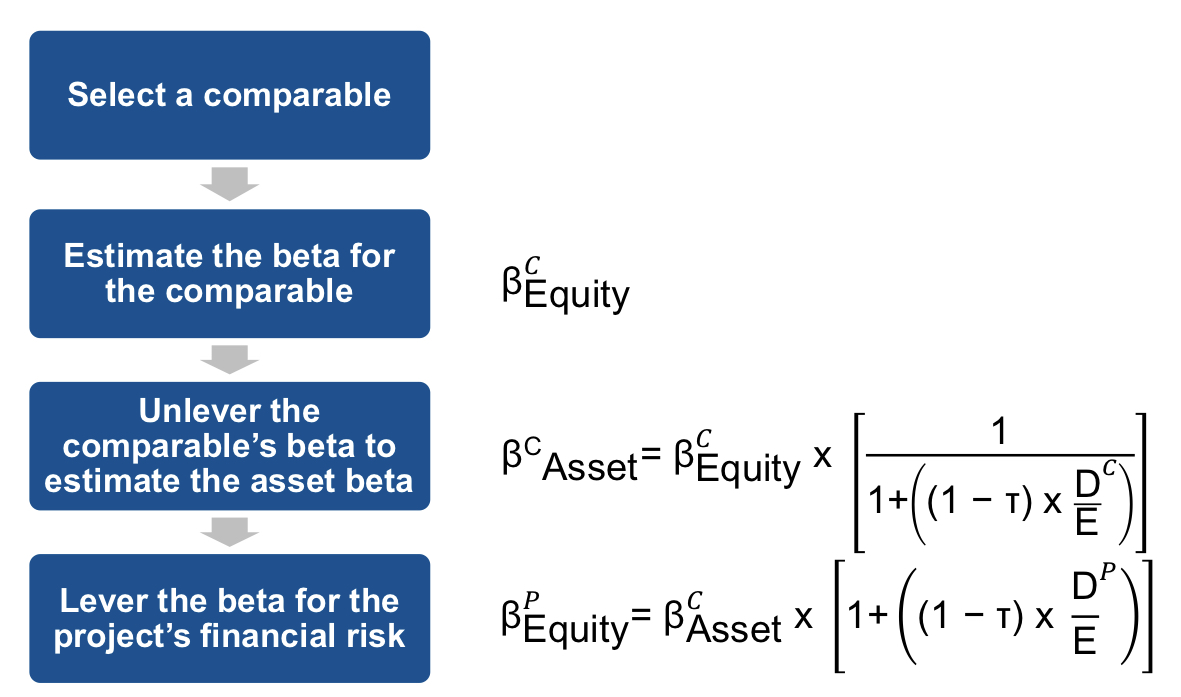
\includegraphics[width=0.6\linewidth]{estimatingbeta.jpg}
		  \label{fig:estimatingbeta_jpg}
		\end{figure}						
						\end{enumerate}
				\end{itemize}
		\end{itemize}
	\end{itemize}
\end{itemize}

\subsection{Debt of cost of capital} % (fold)
\label{sub:debt_of_cost_of_capital}
\begin{itemize}
  \item \textbf{Definition:} It is the effective interest rate that a company pays on its debts, such as bonds and loans.

\item \textbf{Methods of calculating the debt cost of capital:}
	\begin{itemize}
	  \item \textbf{Yield-to-maturity approach:} Debt cost of capital = Yield to maturity on a firm's outstanding debt
	\item \textbf{Debt-rating approach:} Debt cost of capital = Yield based on similarly rated debt (bonds) with similar maturity
	\item \textbf{Beta-CAPM approach:} Debt cost of capital = Expected return for debt based on its beta using CAPM
	\end{itemize}

\item \textbf{Yield-to-maturity approach (YTM):}
	\begin{itemize}
		\item \textbf{Definition:} It is the IRR an investor will earn from holding the bond to maturity\footnote{\textbf{Maturity} is a date on which \underline{a financial agreement ends}, triggering the payment of principal with interest or repayment of a loan with interest.} and receiving its promised payments.

	        \item \textbf{The accuracy of the estimate depends on the risk of firm default!}
			\begin{itemize}
				\item \textbf{Low risk of firm default:} YTM is a reasonable estimate of investors' expected rate of return.
				\item \textbf{High risk of firm default:} YTM will overstate investors' expected return.
			\end{itemize}
	\end{itemize}

\item \textbf{Beta-CAPM approach:}
	\begin{itemize}
		\item Debt betas are difficult to estimate because corporate bonds are traded infrequently.
	\item One approximation is to use estimates of betas of bond indices by rating category.
	\end{itemize}
\end{itemize}

\subsection{A project's cost of capital} % (fold)
\label{sub:a_project_}
\begin{itemize}
  \item \textbf{Should we undertake a given project?}
	  \begin{itemize}
	    \item \textbf{Assumptions:}
		    \begin{itemize}
		      \item All-equity financing of the project separate from any financing decision
			      \item Ignoring financing risk
		    \end{itemize}

\item \textbf{Answer: It depends, especially on project's cost of capital!}
	\begin{itemize}
	  \item To calculate project's cost of capital, we need to find a comparable company and estimate the cost of capital of assets as a proxy.
		  \begin{itemize}
		    \item All-equity firm comparables (company operating by using its \underline{equity})
		    \item Levered firm comparables (company operating by taking out \underline{loans})
		  \end{itemize}
	\end{itemize}
	  \end{itemize}
\item \textbf{All-equity financing: Asset (unlevered) beta}
	\large
	\begin{equation*}
	\boxed{
	\begin{aligned}
	\beta_U = \beta_E * \frac{E}{E + D} + \beta_D * \frac{D}{E+D}
	\end{aligned}
	}
	\end{equation*}
	\normalsize
	
\item \textbf{Levered firms as comparables: Asset cost of capital / unlevered cost of capital}
	\begin{itemize}
	  \item Expected return required by investors to hold firm's underlying assets.
	\item Weighted average of firm's equity and debt costs of capital
	\end{itemize}
	\large
	\begin{equation*}
	\boxed{
	\begin{aligned}
	r_U = r_E * \frac{E}{E + D} + r_D * \frac{D}{E + D}
	\end{aligned}
	}
	\end{equation*}
	\normalsize

\item \textbf{Cash and net debt:}
	\begin{itemize}
	  \item Some items maintain high cash balances.
	\item Cash is a risk-free asset that reduces the average risk of the firm's assets.
	\item Since the risk of the firm's enterprise value is what we are concerned with, leverage should be measured in terms of net debt: \\ \\
		\large
		\boxed{D = Net \; debt = Debt - Excess \; cash \; and \; short-term \; investments}
  \end{itemize}

\item \textbf{Industry asset beta (unlevered beta):}
	\begin{itemize}
	  \item After adjusting for the leverage of different firms to determine their asset betas, we can combine estimates of asset betas for multiple firms in same industry.
		  \item Doing this will reduce estimation error of estimated beat for the project.
	\end{itemize}
\end{itemize}

\subsection{Project risk characteristics and financing} % (fold)
\label{sub:project_risk_characteristics_and_financing}

\begin{itemize}
  \item \textbf{Differences in project risk:}
	\begin{itemize}
	  \item Firm asset betas reflect market risk of the average project in a firm.
	\item Individual projects may be more or less sensitive to market risk.
	\item Financial managers in multi-divisional firms should evaluate projects based on asset betas of firms in a similar line of business.
	\item Another factor that can affect market risk of a project is its degree of operating leverage:
		\begin{itemize}
		  \item Operating leverage is relative proportion of fixed vs.\ variable costs.
		\item A higher proportion of fixed costs increases sensitivity of the project's cash flows to market risk.
			\begin{itemize}
			\item Project's beta will be higher.
			\item A higher cost of capital should be assigned.
			\end{itemize}
		\end{itemize}
	\end{itemize}

\item \textbf{Weighted average of cost of capital (WACC):}
        \begin{itemize}
          \item \textbf{Perfect capital markets:} where, the choice of financing does not affect cost of capital or project NPV, no trader has the power to change the price of goods or services
	\item \textbf{Taxes -- A big imperfection:} When interest payments on debt are tax deductible, net cost to the firm is given by: \\ \\
		\boxed{Effective \; after-tax \; interest \; rate = r * (1 - t_C)}
        \end{itemize}
\item \textbf{WACC Formula:}
	\large
	\begin{equation*}
	\boxed{
	\begin{aligned}
		r_{WACC} = r_E * \frac{E}{E + D} + r_D * \frac{D}{E + D} * (1 - t_C)
	\end{aligned}
	}
	\end{equation*}
	\normalsize

\item \textbf{Given a target leverage ratio:}
	\large
	\begin{equation*}
	\boxed{
	\begin{aligned}
		r_{WACC} = r_U - \frac{D}{E + D} * t_C * r_D
	\end{aligned}
	}
	\end{equation*}
	\normalsize
	
\item \textbf{r\textsubscript{WACC} vs.\ r\textsubscript{U}:}
	\begin{itemize}
		\item Unlevered cost of capital (or pre-tax WACC) = r\textsubscript{U}
			\begin{itemize}
			  \item Expected return investors will earn by holding firm's assets.
			\item In a world with taxes, it can be used to evaluate an all-equity with the same risk as the firm.
			\end{itemize}
		\item In a world with taxes, WACC is less than the expected return of firm's assets.
			\begin{itemize}
			 \item With taxes, WACC can be used to evaluate a project with the same risk and the same financing as the firm. 
			\end{itemize}
	\end{itemize}
\end{itemize}

\section{Capital Structure} % (fold)
\label{sec:capital_structure}

\subsection{Equity vs.\ debt financing} % (fold)
\label{sub:equity_vs_ debt_financing}

\begin{itemize}
  \item \textbf{Basic question of corporate finance = Capital structure decision:} After the decision whether or not to undertake an investment, which type of security should a firm sell to investors.

\item \textbf{Definition:} The relative proportions of debt, equity, and other securities that a firm has outstanding. Two main types of capital structure:
	\begin{itemize}
	  \item \textbf{Financing a firm with equity} (= all-equity financing, unlevered firm)
          \item \textbf{Financing a firm with equity and debt} (= levered firm)

	 \item \textbf{Is there a capital structure that shareholders prefer?}
	\end{itemize}
\end{itemize}

\subsection{Modigliani-Miller 1: Leverage and arbitrage} % (fold)
\label{sub:modigliani_miller_1_leverage_and_arbitrage}

\begin{itemize}
  \item \textbf{Capital structure decision:} The theory of capital structure was developed beginning with the capital structure theory of Merton Miller and Franco Modigliani (MM).

\item \textbf{Assumptions of MM model:}
	\begin{itemize}
	  \item \textbf{Homogeneous expectations}
		  \item \textbf{Homogeneous business risk classes}
	\item \textbf{Perpetual cash flows}
	\item \textbf{Perfect capital markets:}
		\begin{itemize}
		  \item Investors and firms can trade the same set of securities at competitive market prices equal to the present value of their future cash flows.
		\item No taxes, transaction costs, issuance costs or agency costs associated with security trading
		\item A firm's financing decisions do not change the cash flows generated by its investments, nor do they reveal new info about them.
		\end{itemize}
	\end{itemize}

\item \textbf{Modigliani and Miller argue:} In a perfect capital market, total value of a firm is equal to the market value of the total cash flows generated by its assets and is not affected by its choice of capital structure. \underline{Reasons:}
\begin{itemize}
  \item Market value of any firm is independent of its capital structure.
\item If a company has a given set of assets, changing debt to equity will change the way net operating income is divided between lenders and shareholders, but will not change the value of the company.
 
\end{itemize}

\item \underline{\textbf{MM proposition 1 (without taxes):}} \textbf{The market value of a company is not affected by the capital structure of the company.}
	\large
	\begin{equation*}
	\boxed{
	\begin{aligned}
	E + D = U = A
	\end{aligned}
	}
	\end{equation*}
	\\
	\normalsize
	With:\\
	E = Market value of equity in a levered firm, D = Market value of debt in a levered firm, U = Market value of equity in an unlevered firm, A = Market value of the firm's assets

\item \textbf{Proof of MM proposition 1:}
	\begin{itemize}
	  \item \textbf{Law of one price:} Firm's securities and its assets need to have the same total market value.
		  \begin{itemize}
			  \item Otherwise, an arbitrage\footnote{\textbf{Arbitrage} is the simultaneous purchase and sale of the \underline{same asset in different markets} in order to profit from tiny differences in the asset's listed price.} opportunity would exit.
		  \end{itemize}
\item \textbf{Homemade leverage:} The investors use leverage in their own portfolios to adjust the leverage choice made by the firm.
	\begin{itemize}
	  \item Homemade leverage is a perfect substitute for corporate leverage
	\item Substitutability between corporate debt and personal debt
	\end{itemize}
	\end{itemize}
\item \textbf{A leveraged recapitalization: Application of MM proposition 1}
	\begin{itemize}
	  \item How do firms adjust their capital structure?
	\item A firm can use borrowed funds to pay a large special dividend or repurchase a significant amount of outstanding shares.
  \end{itemize}
\end{itemize}

\subsection{Modigliani-Miller 2: Leverage and cost of capital} % (fold)
\label{sub:modigliani_miller_2_leverage_and_cost_of_capital}



% subsection modigliani_miller_2_leverage_and_cost_of_capital (end)
% subsection modigliani_miller_1_leverage_and_arbitrage (end)
% subsection equity_vs_ debt_financing (end)


% section capital_structure (end)
% subsection project_risk_characteristics_and_financing (end)

% subsection a_project_ (end)
% subsection debt_of_cost_of_capital (end)	   
							% subsection equity_of_cost_of_capital (end)

% section cost_of_capital (end)
% subsection  (end)


% subsection risk_analysis (end)



% subsection further_adjustments_to_fCF (end)



% subsubsection choosing_among_alternatives (end)
% subsubsection determining_free_cash_flow_fCF_and_nPV (end)



% subsection capital_budgeting (end)

% subsubsection other_methods (end)
% subsubsection internal_rate_of_return_iRR_ (end)
% subsubsection net_present_value_nPV_ (end)

% subsection investment_analysis (end)


% subsubsection  (end)
% subsubsection statement_of_cash_flows (end)

% subsubsection subsubName (end)


\end{document}
